\chapter{Experimental Methods}

\begin{figure}[h]
  \centering
  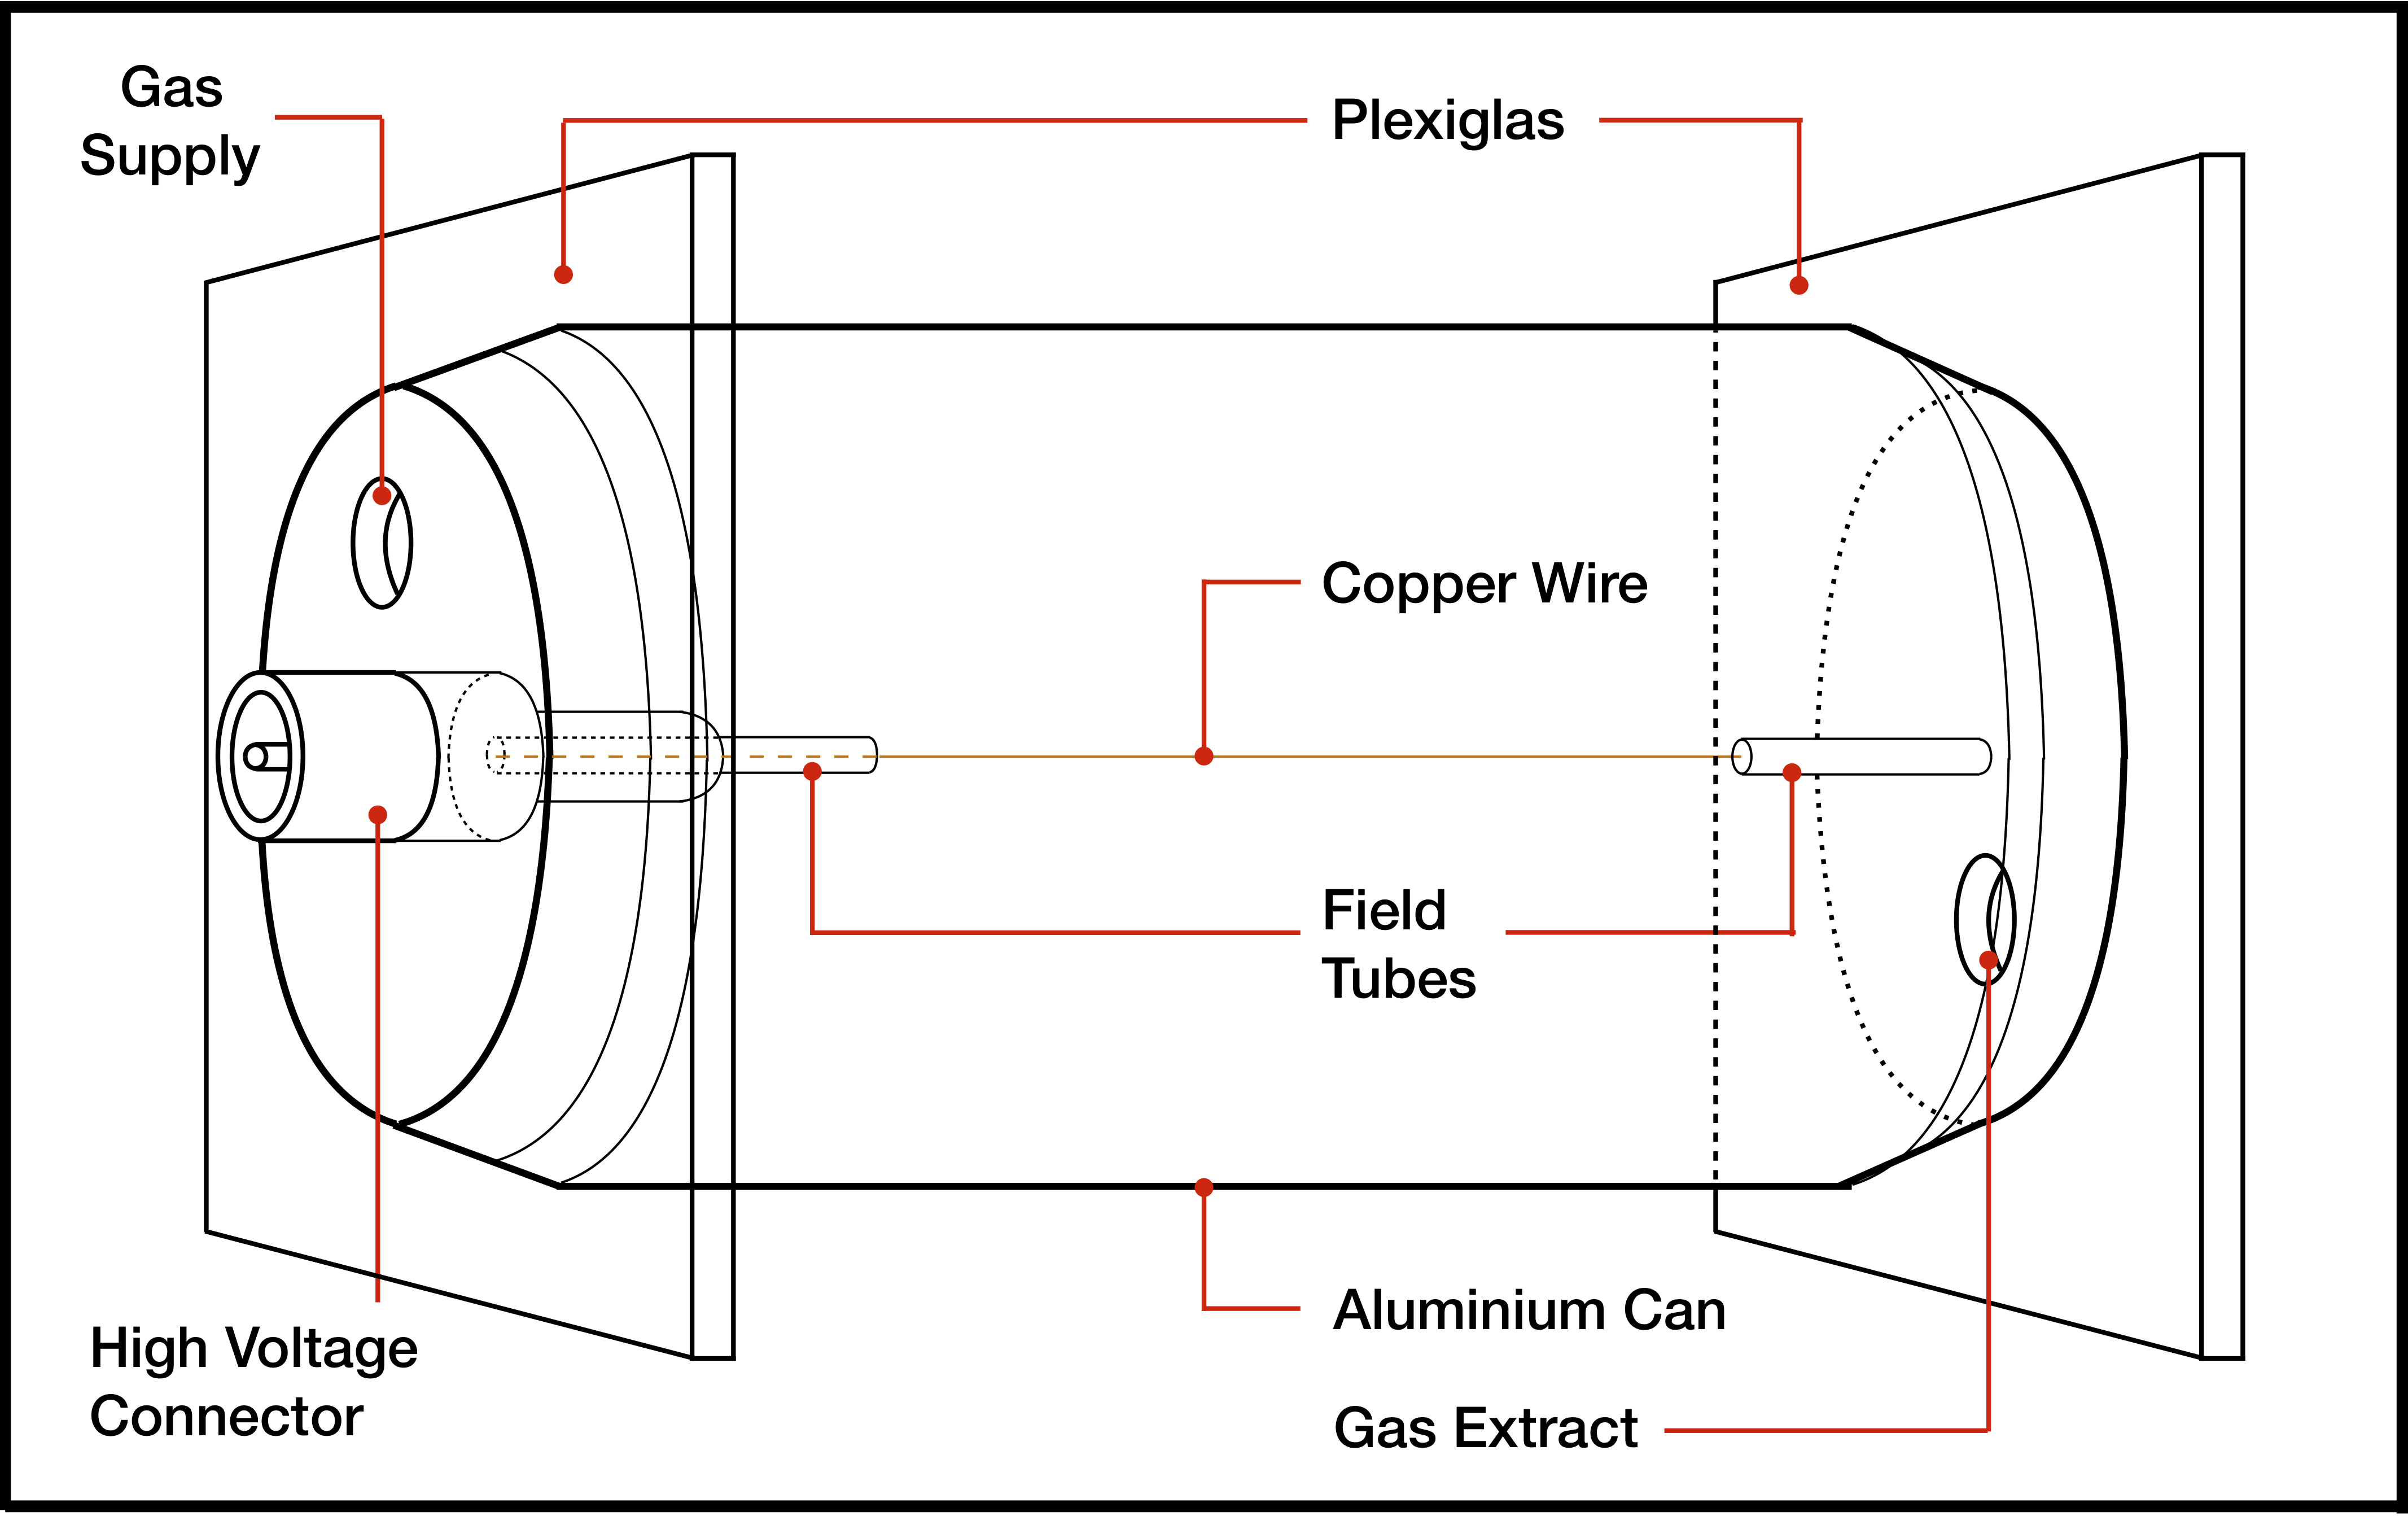
\includegraphics[width=\textwidth]{detectorSchematic.png}
  \caption{Schematic of the detector.}
  \label{fig:schematic}
\end{figure}

\section{Detector Assembly}

For the cathode, an aluminium beverage can was used. The ends were removed using a hole saw drill bit, and filed down with a rat-tail file to ensure there were no sharp points from which sparking could occur. The non-conducting oxide layer on the interior of the can was removed with a stiff sponge attached to a battery powered drill. On the can's exterior, a strip of paint was sanded away with abrasion paper so that an electrical contact to ground could be established. Connectivity was tested with a digital multi-meter to check that the insulating layer had been completely removed. If it was not, the shape of the electric field inside of the detector would not have followed the cylindrical geometry used in the Diethorn formula (Equation \ref{eqn:Diethorn}).

The can's length and diameter were found to be inconsistent when measured at corresponding points around the can. Three measurements were made to give an average and standard error, which exceeded the instrumental uncertainty in both cases. The length and diameter were found to be (111.00$\pm$0.09)mm and (52.8$\pm$0.1)mm respectively. The can wall was directly measured as (0.22$\pm$0.01)mm, however due to the curvature of the can this was not representative of the can wall thickness. By also measuring the diameter of the micrometer spindle and using some simple geometry a rough value for the thickness of the can was found as (0.02$\pm$0.05)mm, however the uncertainty is greater than the value itself and so cannot be trusted.

The ends of the can were covered by Plexiglas endplates, with grooves cut for the can to slot into. Holes were drilled in the endplates: a 9.4mm drill bit was used for the HV connector, 1.0mm for the field tubes and 5.6mm for gas pipes.

A single copper thread was taken from an ordinary braided electrical cable to use as the anode, this had a diameter of approximately (50$\pm$10)\textmu m. Both pieces of field tube were cut from the same length of brass tube with a manufacturer's diameter of 1mm. They were also filed at both ends to prevent sparking. After they had been filed, their lengths were measured as (26.87$\pm$0.02)mm and (13.75$\pm$0.02)mm. A commercial high voltage connector was used to connect the detector to the preamplifier.

Once all the components were prepared and ready for assembly, they were cleaned in isopropanol in an ultrasonic bath for two minutes. This is to remove any dust, grease or flakes of metal which may have accumulated on the components during their preparation. From this point onwards, gloves were worn to keep the components clean.

\begin{figure}[h]
  \centering
  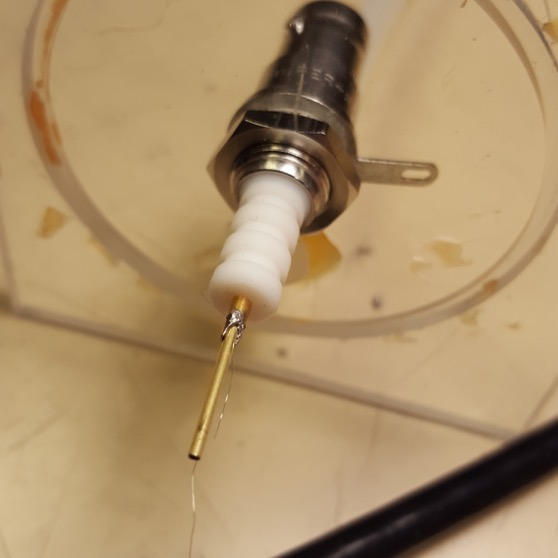
\includegraphics[width=7cm]{HVconnector.jpg}
  \caption{Photograph showing the connection between the anode, field tube, high voltage connector and endplate.}
  \label{fig:HVC}
\end{figure}

The anode was threaded through the shorter field tube until a short length was poking out of the other side. The field tube was then inserted into the high voltage connector with the short length of anode hanging loose outside of the connector. The components were soldered together where the field tube and anode emerged from the high voltage connector securing both in place. The high voltage connector was in turn connected to the endplate using a bolt supplied with the connector (Figure \ref{fig:HVC}).

To glue the components together Araldite glue was used as it also forms an airtight seal around the joints, preventing gas leaks. The longer field tube was glued in the endplate with the 1mm hole, and the anode was threaded through the shielding so that it could be soldered on the other side. Both endplates were taped onto the detector to hold them in place while the anode was pulled taut and soldered -- in case it snapped and the detector needed to be reopened. Once the anode was soldered it was checked to ensure it was taut which is important for ensuring a uniform electric field inside the detector. The endplates were then glued to the can and the gas supply tubes were glued into the endplates. Glue was also applied around the high voltage connector and the free end of the anode to seal the detector.

To reduce noise; insulating Kapton tape was stuck over the free end of the detector. Copper tape was also stuck from the high voltage connector to the conducting strip on the outside of the aluminium can. Finally aluminium shielding was folded around the endplates and grounded by a cable from the high voltage connector (Figure \ref{fig:setup}).

\section{Measurements}

\begin{figure}[h]
  \centering
  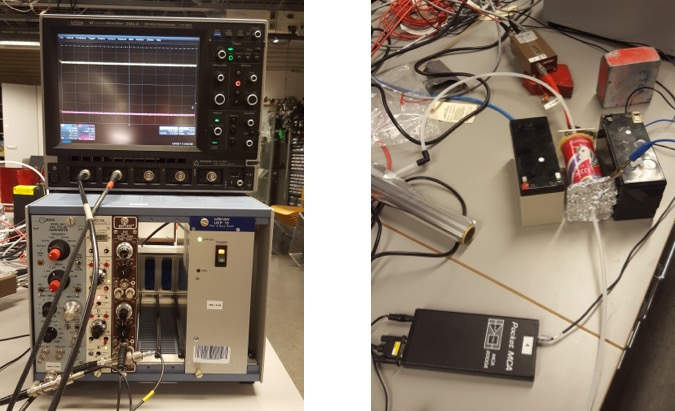
\includegraphics[width=\linewidth]{apparatus.jpg}
  \caption{Photographs of the apparatus used to perform the experiment. Seen in the picture is the Wiener UEP 15 (Power Supply), ComTec MHQ206L (High Voltage Supply), ORTEC 855 Dual Amplifier (Spectroscopic Amplifier), BNC Model BH-1 (Pulse Generator), LeCroy Wavesurfer 24Xs-A (Oscilloscope), ORTEC 142A (Preamplifier) and Amptek MCA8000A (Multichannel Analyser).}
  \label{fig:setup}
\end{figure}

The detector needs to be flushed with P-10 gas before any measurements can be taken, so the seal of the detector was checked first using a gas flow meter. The gas flow supplied to the detector was measured as (10.3$\pm$0.2)ml/min and the gas flow out of the detector was found to be (9.9$\pm$0.2)ml/min which means the detector was sufficiently gas tight. The gas flow was then turned up to reduce the amount of time taken to flush the detector and left for several hours. Once the detector had been satisfactorily flushed, the gas flow was reduced back down to a flow rate of (18.4$\pm$0.2)ml/min.

The detector was connected to the preamplifier via the high voltage connector, which was in turn connected to the high voltage supply and pulse generator. The multichannel analyser was set to measure over the voltage range 10V sorting into 512 bins. Higher resolution is unnecessary since the detector resolution is the limiting factor. The pulse generator, high voltage supply and spectroscopic amplifier (spec amp) were powered by the Wiener power supply to regulate the current and voltage supply to the instruments.

An aluminium collimator was used for taking any measurements using the \textsuperscript{55}Fe source. For the \textsuperscript{241}Am source a lead collimator was used to further reduce the number of gamma rays entering the detetcor per unit time. This is because \textsuperscript{241}Am is a very high activity source and the response time of the detector is too slow to record each gamma ray as an individual event. When using the \textsuperscript{241}Am source a lead shield was also positioned around the detector to minimise exposure to those in the lab.

\subsection{Electron Calibration}

\begin{figure}[h]
  \centering
  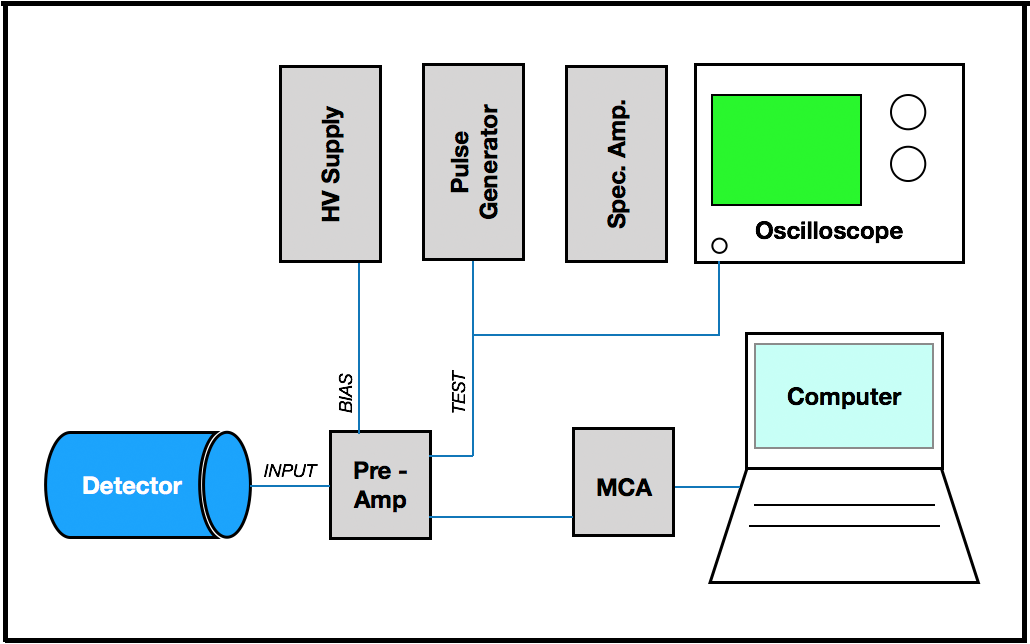
\includegraphics[width=\linewidth]{calibrationSchematic.png}
  \caption{Diagram showing the experimental setup for performing the electron calibration.}
  \label{fig:calibrationSetup}
\end{figure}

To characterise the detector, one must know what MCA channel number corresponds to what detected charge. The pulse generator output was split using a \textquotesingle T\textquotesingle \space connector and connected to the oscilloscope and preamplifier as shown in Figure \ref{fig:calibrationSetup}. The output of the preamplifier was fed straight to the MCA and the high voltage supply was left off. The pulse generator sent pulses to the preamplifier with a rise time of 50ns and a fall time of 50\textmu s to mimic the pulse shape of ionisation events in the detector. The average voltage of the pulses and their standard deviation were measured on the oscilloscope using its built in measurement function. The MCA measured the signal for 10 seconds, sorting the pulses into 512 bins to be displayed on the spectrum software. These measurements were repeated at 10mV intervals from 10mV until 150mV where the pulse exceeded the MCA's 10V limit. This resulted in a series of sharp peaks ranging across the MCA channels (Figure \ref{fig:electronCalibrationData}). The centre, its uncertainty and the full width at half maximum (FWHM) of each peak was then fitted in the software using the built in fitting tool (Table \ref{tbl:electronCalibrationData}).

The preamplifier had a capacitance of 1pF which made it possible to calculate the collected charge from the measured voltage, which in turn enabled the number of collected electrons to be calculated:
\begin{equation}
    C = \frac{Q}{V}
    \label{eqn:C=Q/V}
\end{equation}
\begin{equation}
    n_e = \frac{Q}{e}
    \label{eqn:n_e}
\end{equation}

The errors in the input pulse voltage arose from both statistical error and instrumental error. The statistical error is a result of the spread of values as measured by the oscilloscope, and the instrumental error is specified by the manufacturer as $\pm$1\% of the full scale. Since the full scale was not recorded for each measurement, it will be estimated as $\pm$3\% of the measured pulse voltage because the signal never spanned less than 1/3 of the total scale. These errors were added by quadrature.

Error in the channel also arose due to non-linearities and temperature instability in the preamplifer and MCA, resulting in an error of $\pm$0.185\%. This is insignificant compared to the error from the fit, but was included in calculations for completeness. It was added to the error given by the specutrum software's fitting tool by quadrature.

This data was then plotted and fitted using Python's ODR package, which takes x and y errors into account, to two linear models: one with a constant term and one without. One would expect there to be no constant term since channel number should read zero when the pulse voltage is zero, and the uncertainty for the constant term when fitted is very large compared to its actual value, which supports this (Figure \ref{fig:calibration}). For this reason the model with no constant term was used to produce the calibration equation.

\subsection{Voltage Scan} \label{sec:mthd:voltageRun}

\begin{figure}[h]
  \centering
  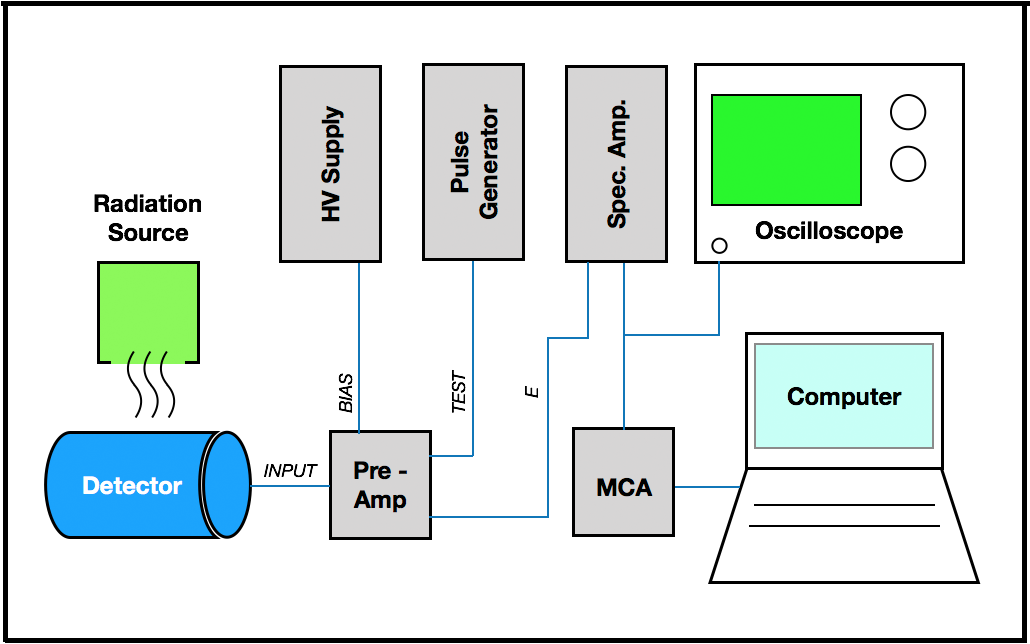
\includegraphics[width=\linewidth]{scanSchematic.png}
  \caption{Diagram showing the experimental setup for performing the voltage scan.}
  \label{fig:scanSetup}
\end{figure}

To test the proportionality of the detector, the collected charge was measured as a function of applied voltage. To perform these measurements the pulse generator was turned off and the high voltage supply was turned on. The signal from the preamplifier was now sent to a spec amp which was set to its maximum gain, and was then split between the oscilloscope and the MCA using a \textquotesingle T\textquotesingle connector.
The high voltage supply was then gradually increased until a signal was observed on the oscilloscope. For \textsuperscript{55}Fe this was observed at 1520V.

The spectrum was then measured for 60 seconds at 50V increments on the high voltage power supply. The spectrum software was used to fit to \textsuperscript{55}Fe's main photopeak, giving the peak centre, its uncertainty and the FWHM. When the spectrum filled the MCA's channels; without changing the voltage, the coarse gain was reduced by one increment so that systematic errors arising from nonlinearities in the spec amp coarse gain could be estimated. This was repeated until spectrum filled the MCA channels at the lowest spec amp gain.

The \textsuperscript{55}Fe sample and aluminium collimater were then swapped for the \textsuperscript{241}Am and lead collimator, and the voltage was reduced until the spectrum fitted in the MCA's channel range. Working in the opposite direction to before, the spectrum was then measured for 180 seconds before reducing the high voltage supply in 50V increments, taking the same measurements as before. When the spectrum filled only the lower channels of the MCA, the coarse gain was increased and the process repeated until the coarse gain was at its maximum.

Using the channel number and the conversion equation, the number of detected electrons from the \textsuperscript{55}Fe and \textsuperscript{241}Am photopeaks can be plotted against the high voltage supply.

Error in the high voltage scan came from fluctuations in the readout during the measurement of $\pm$1V. There was also instrumental error specified by the manufacturer of $\pm$(0.05\%V + 0.02\%V\textsubscript{max} + 1 digit per year), where V is the measured voltage in kV, V\textsubscript{max} is the maximum voltage in kV (6kV for this instrument) and 1V was added since the high voltage supply was one year old. These two uncertainties were added by quadrature.

Error in the number of detected electrons came from the statistical error from the spectrum software fit and instrumental error from the preamplifier and MCA as before, but this time the spec amp gain is changed and therefore contributes to the error as well. The spec amp has errors stated by the manufacturer attributed to non-linearities (which are not important as fine gain was not changed) and temperature instability. As well as these, it can be seen that there are discontinuities in the number of detected electrons when the coarse gain is changed. This error was taken into account by summing the absolute value of the discontinuities in channel number over the whole range of measurements. Choosing to use a constant error was motivated by the fact that the size of the error did not increase in size at higher gains and there is no reason to believe the spec amp is more accurate at a lower gain. These two errors were added by quadrature.

\subsection{Multiplication Factor}

To calculate the multiplication factor, the ratio of electrons produced in the detector to the number of electrons produced in the original ionisation event must be determined. The number of electrons produced in the detector was calculated when performing the voltage run so this number simply needs to be divided by the number of original ions, given by Equation \ref{eqn: n_0}.

A book value was used for W \cite{Wolff_W_dV_K} which has no uncertainty quoted so the only uncertainty in the multiplication factor calculation is carried through from the uncertainty in the number of detected electrons:
\begin{equation}
    \Delta M = \frac{\Delta n_{e}}{n_{i}}
\end{equation}

The theoretical Diethorn equation (Equation \ref{eqn:Diethorn}) was plotted on the same graph, using book values for $\Delta$V and K \cite{Wolff_W_dV_K}. The uncertainty limits are given by:
\begin{equation}
    \lambda = \ln{\bigg( \frac{b}{a} \bigg)}
\end{equation}
\begin{equation}
    \Delta \lambda = \sqrt{\bigg(\frac{\Delta a}{a}\bigg)^{2} + \bigg(\frac{\Delta b}{b}\bigg)^{2}}
\end{equation}
\begin{equation}
    \zeta = \ln{\bigg(\frac{V}{paK\lambda}\bigg)}
\end{equation}
\begin{equation}
    \Delta \zeta = \sqrt{\bigg(\frac{\Delta V}{V}\bigg)^{2} + \bigg(\frac{\Delta p}{p}\bigg)^{2} + \bigg(\frac{\Delta a}{a}\bigg)^{2} + \bigg(\frac{\Delta K}{K}\bigg)^{2} + \bigg(\frac{\Delta \lambda}{\lambda}\bigg)^{2}}
\end{equation}
\begin{equation}
    \Delta M = M \cdot \sqrt{\bigg(\frac{\Delta V}{V}\bigg)^{2} + \bigg(\frac{\Delta \lambda}{\lambda}\bigg)^{2} + \bigg(\frac{\Delta (\Delta V)}{(\Delta V)}\bigg)^{2} + \bigg(\frac{\Delta \zeta}{\zeta}\bigg)^{2}}
\end{equation}

\subsection{Energy Resolution}

To calculate the energy resolution of the detector, the ratio of the full width at half maximum (FWHM) to centroid channel is taken. Using the data collected in the voltage run, a graph was plotted of FWHM against centroid channel, both corrected for gain, for \textsuperscript{55}Fe and \textsuperscript{241}Am. This way it was easy to identify whether spec amp gain has an impact on the energy resolution. A straight line with no constant term was fitted to the plots, taking into account centroid channel uncertainty, and the gradient was the energy resolution (Figures \ref{fig:energyResolutionFe}, \ref{fig:energyResolutionAm}).

A separate graph was also plotted to determine whether there is any correlation between energy resolution and applied voltage.

\subsection{Spectra} \label{sec:mthd:spectra}

The spectra of both \textsuperscript{55}Fe and \textsuperscript{241}Am were measured with their respective collimators, an applied voltage of (1777$\pm$5)V and a spec amp gain of 10. The \textsuperscript{55}Fe source was measured for 313 seconds and the \textsuperscript{241}Am source for 374 seconds. The spectra could be normalised by plotting in terms of intensity (counts divided by measurement time).

The \textsuperscript{55}Fe spectrum resembles two Gaussian curves and python's non-linear least squares algorithm was used to fit a model consisting of two Gaussian curves and a constant background. This gave a good fit however as previously discussed (Chapter \ref{sec:intr:radiationSources}), the main photopeak actually consists of two superimposed peaks a new model was fitted consisting of three Gaussian curves and a constant background, proving to be an even better fit.

It was harder to fit peaks to the \textsuperscript{241}Am spectrum which had a far more complex spectrum. The spectrum was taken to WebPlotDigitizer where an estimate of the background was traced from the original spectrum. This was modelled by two exponential functions multiplied by a fermi function:
\begin{equation}
    Background = (a_{1}e^{b_{1}x}+a_{2}e^{b_{2}x})(1+e^{\frac{x-c}{d}})^{-1}
\end{equation}
This was fitted using python's non-linear least squares algorithm and this background curve was subtracted from the original spectrum leaving just the peaks. The necessary parameters for Gaussian curves were estimated for each of the 5 peaks. Finally, a model was built from the background model plus five Gaussian curves. The parameters previously estimated were used as first guess values and the complete model was successfully fitted with improved accuracy for the parameters.

The fitted peaks were labelled from 1-3 for the \textsuperscript{55}Fe spectrum and from 4-8 for the \textsuperscript{241}Am spectrum, in ascending order of 
channel number (Figures \ref{fig:Fe55spec}, \ref{fig:Am241spec}).

\subsection{Energy Calibration}

As a result of fitting gaussian curves to the spectra, the centres all the spectral peaks are now known. Some of these peaks are very well defined and can be used to determine the relationship between channel number and radiation energy.

Peak 1 is the argon escape peak which has an energy of 3.19keV. Peaks 2 and 3 can be attributed to the relaxation of \textsuperscript{55}Fe's daughter nucleus \textsuperscript{55}Mn with energies of 5.89keV and 6.42keV respectively. Peak 8 produced by a transition in \textsuperscript{241}Am's daughter nucleus \textsuperscript{237}Np which prodcues a gamma ray with an energy of 59.54keV.

By modelling the relationship between peak centre channels against their energies as a straight line, a conversion equation can be determined (Figure \ref{fig:energyCalibration}).

\section{Preamplifier}

\begin{figure}[h]
  \centering
  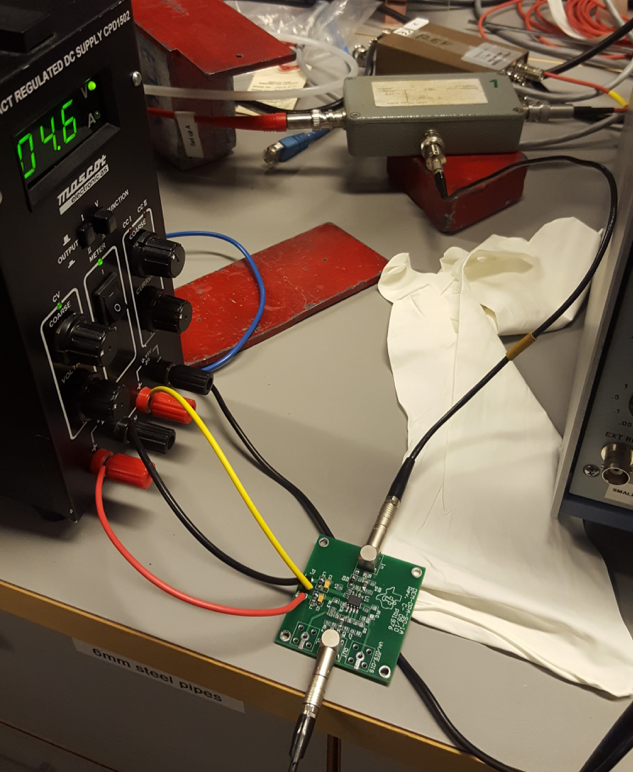
\includegraphics[width=9cm]{preampSpectrumSetup.png}
  \caption{Experimental setup using the kit preamplifier to measure the spectrum of \textsuperscript{55}Fe.}
  \label{fig:preampSpecSetup}
\end{figure}

The preamplifer was assembled from a kit produced by Texas Instruments. The resistors chosen had resistances of 470$\Omega$ and 22$\times10^{6}\Omega$, which gives an expected gain of 46.8.

The gain was checked using the pulse generator and oscilloscope and measuring the ratio of the input pulse voltage from the pulse generator to the output voltage from the preamplifier on the oscilloscope.

The same setup was used as for measuring the spectrum as in Section \ref{sec:mthd:spectra}, only the ORTEC preamplifier is replaced with a decoupler. This is uses capacitance decoupling to output only the signal to the kit preamplifier, as seen in Figure \ref{fig:preampSpecSetup}.

The power supply to the preamplifier was turned up to 4.6V, and the \textsuperscript{55}Fe positioned above the detector on its aluminium collimator. The high voltage supply to the detector was ramped up to 2317V and the coarse gain on the spec amp set to 10. The spectrum was measured for 180 seconds. The dominating source of error in this setup is now the preamplifier and can be estimated using the resistor tolerances.

The spectrum was plotted and fitted using a single gaussian fit about the main photopeak, so that the energy resolution could be compared to the \textsuperscript{55}Fe spectrum taken using the ORTEC preamplifier.